\chapter*{Salar d’Uyuni\markboth{Salar d’Uyuni}{}}
\section*{4 avril 2015}
Depuis San Juan direction nord pour rejoindre le Salar d'Uyuni, le plus grand désert de sel du monde. C'est la fin de la saison des pluies et le Salar a eu le temps de sécher pour être praticable en vélo. 

 En 1 jour on arrive à l'entrée du Salar. 

 

\begin{center} 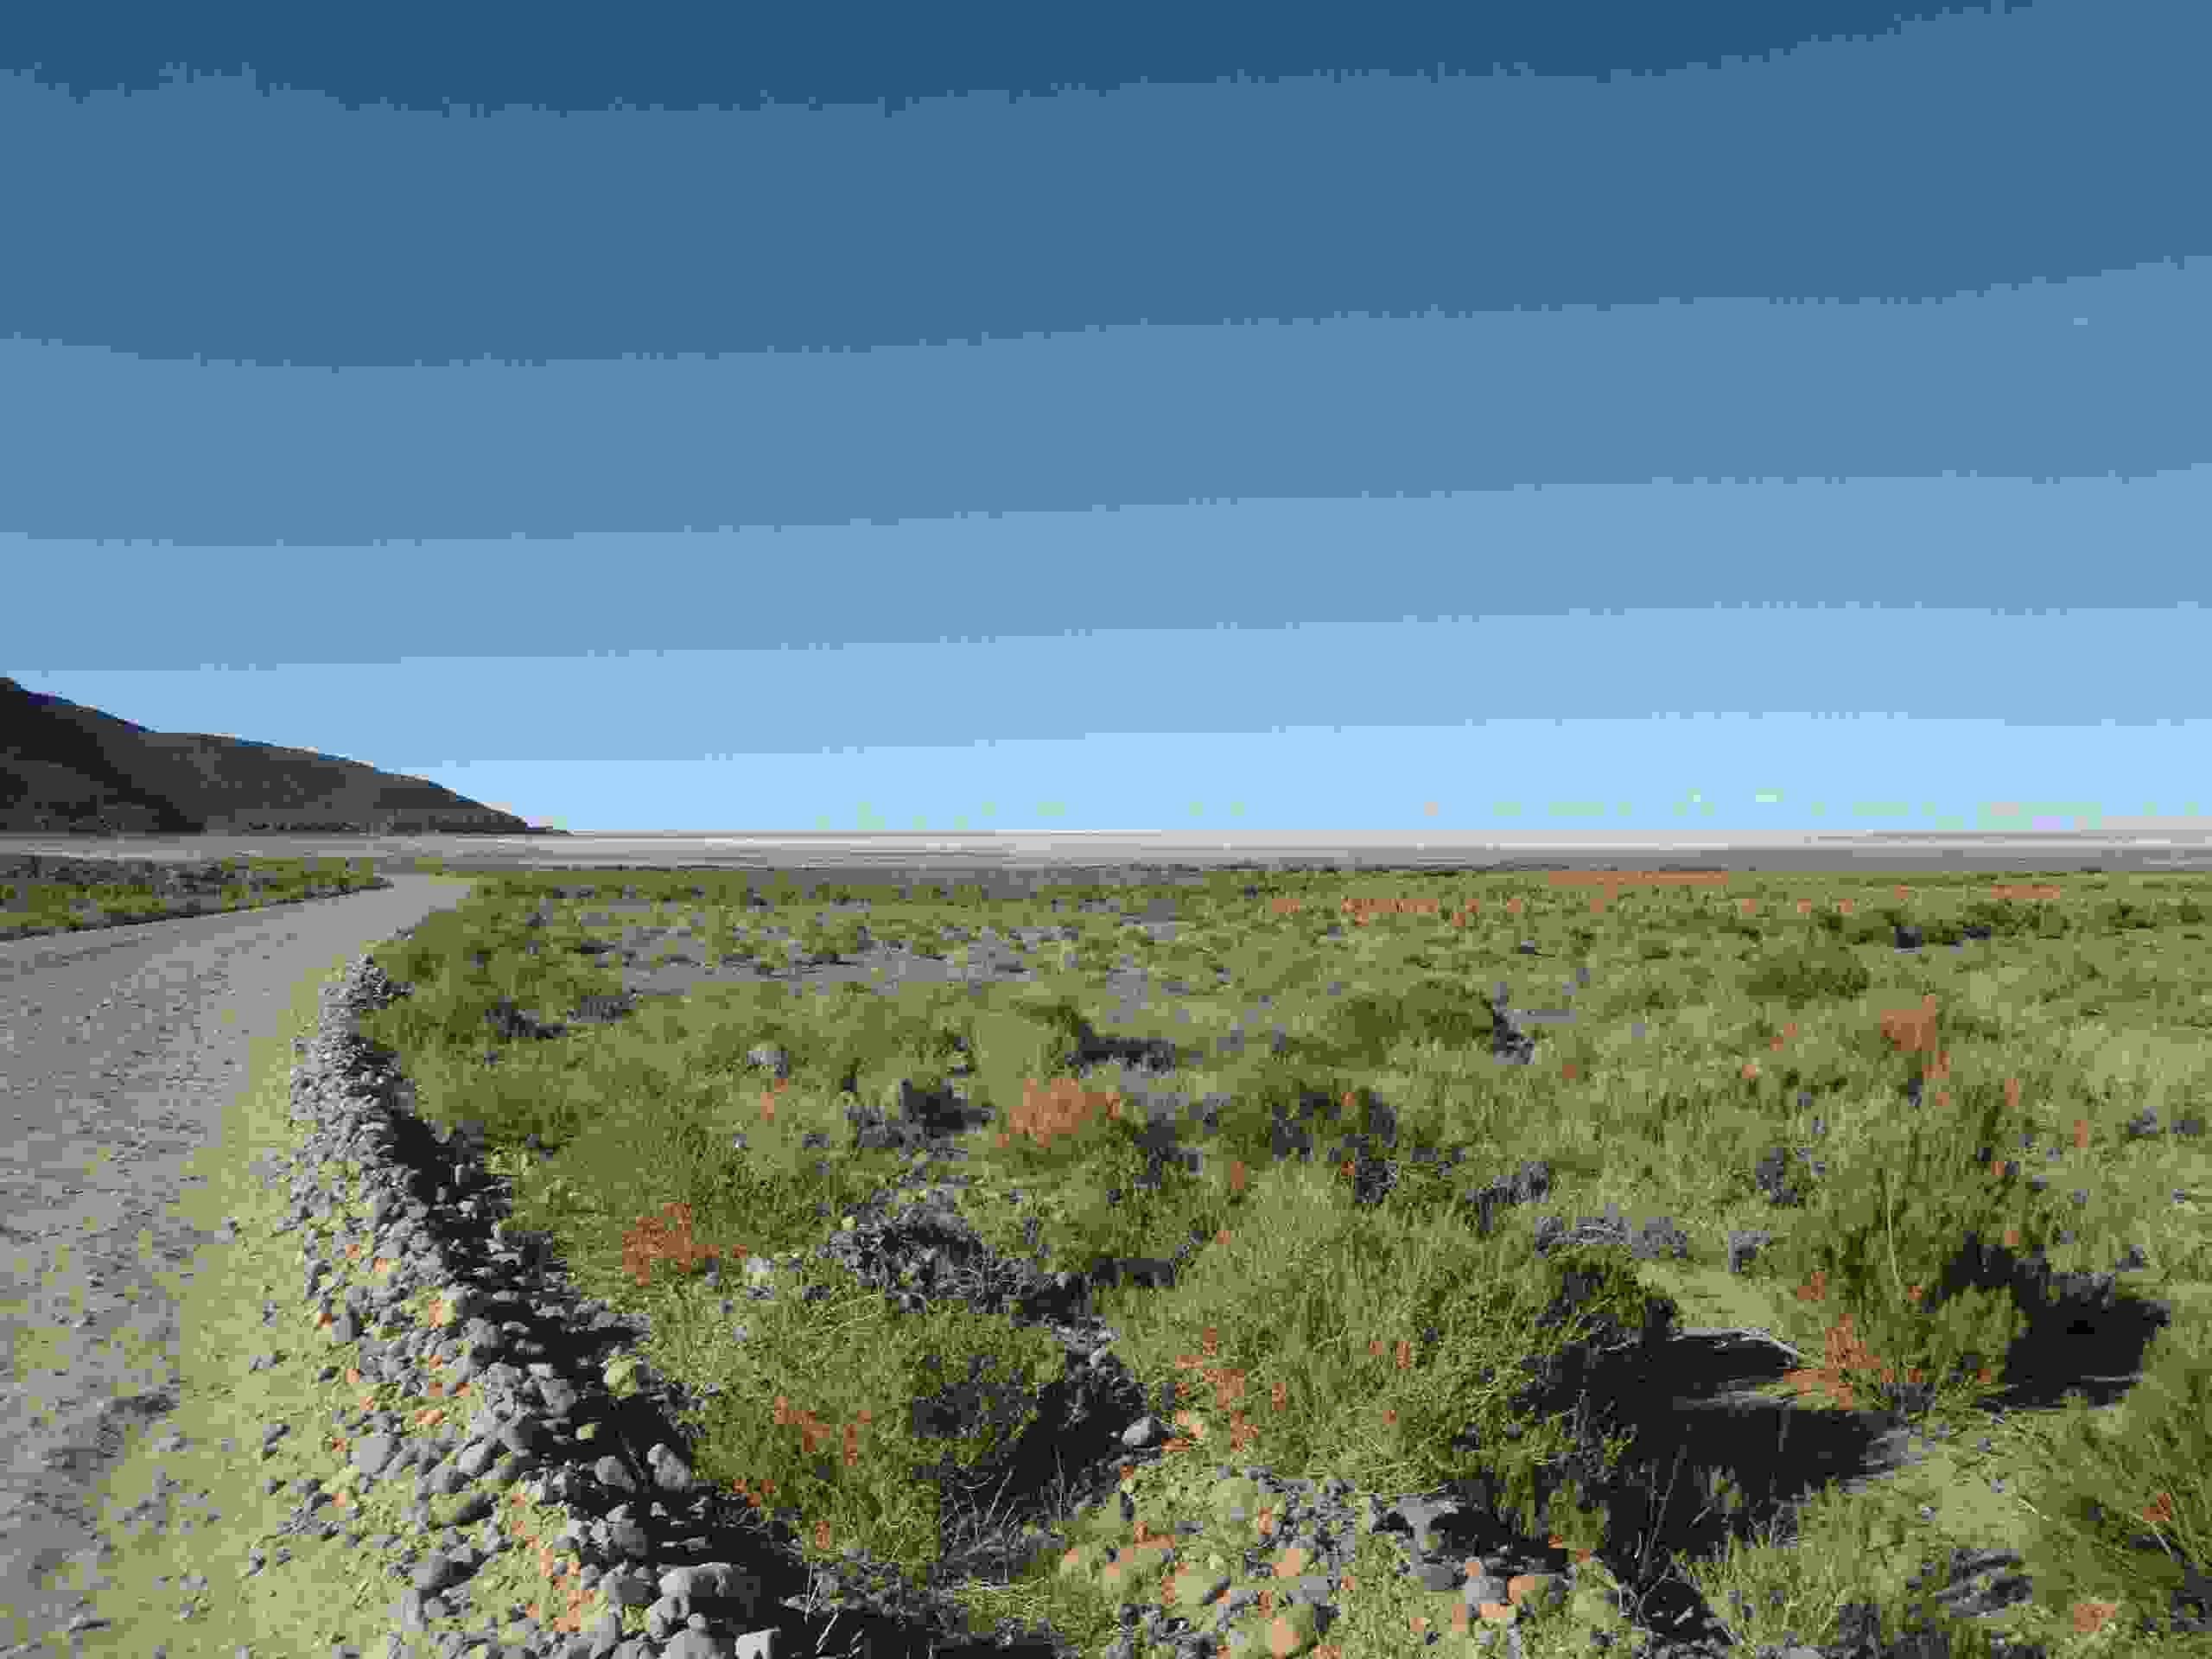
\includegraphics[width=\mywidth]{../wp-content/uploads/2015/04/wpid-wp-1427985910677.jpg} \end{center}



 

\begin{center} 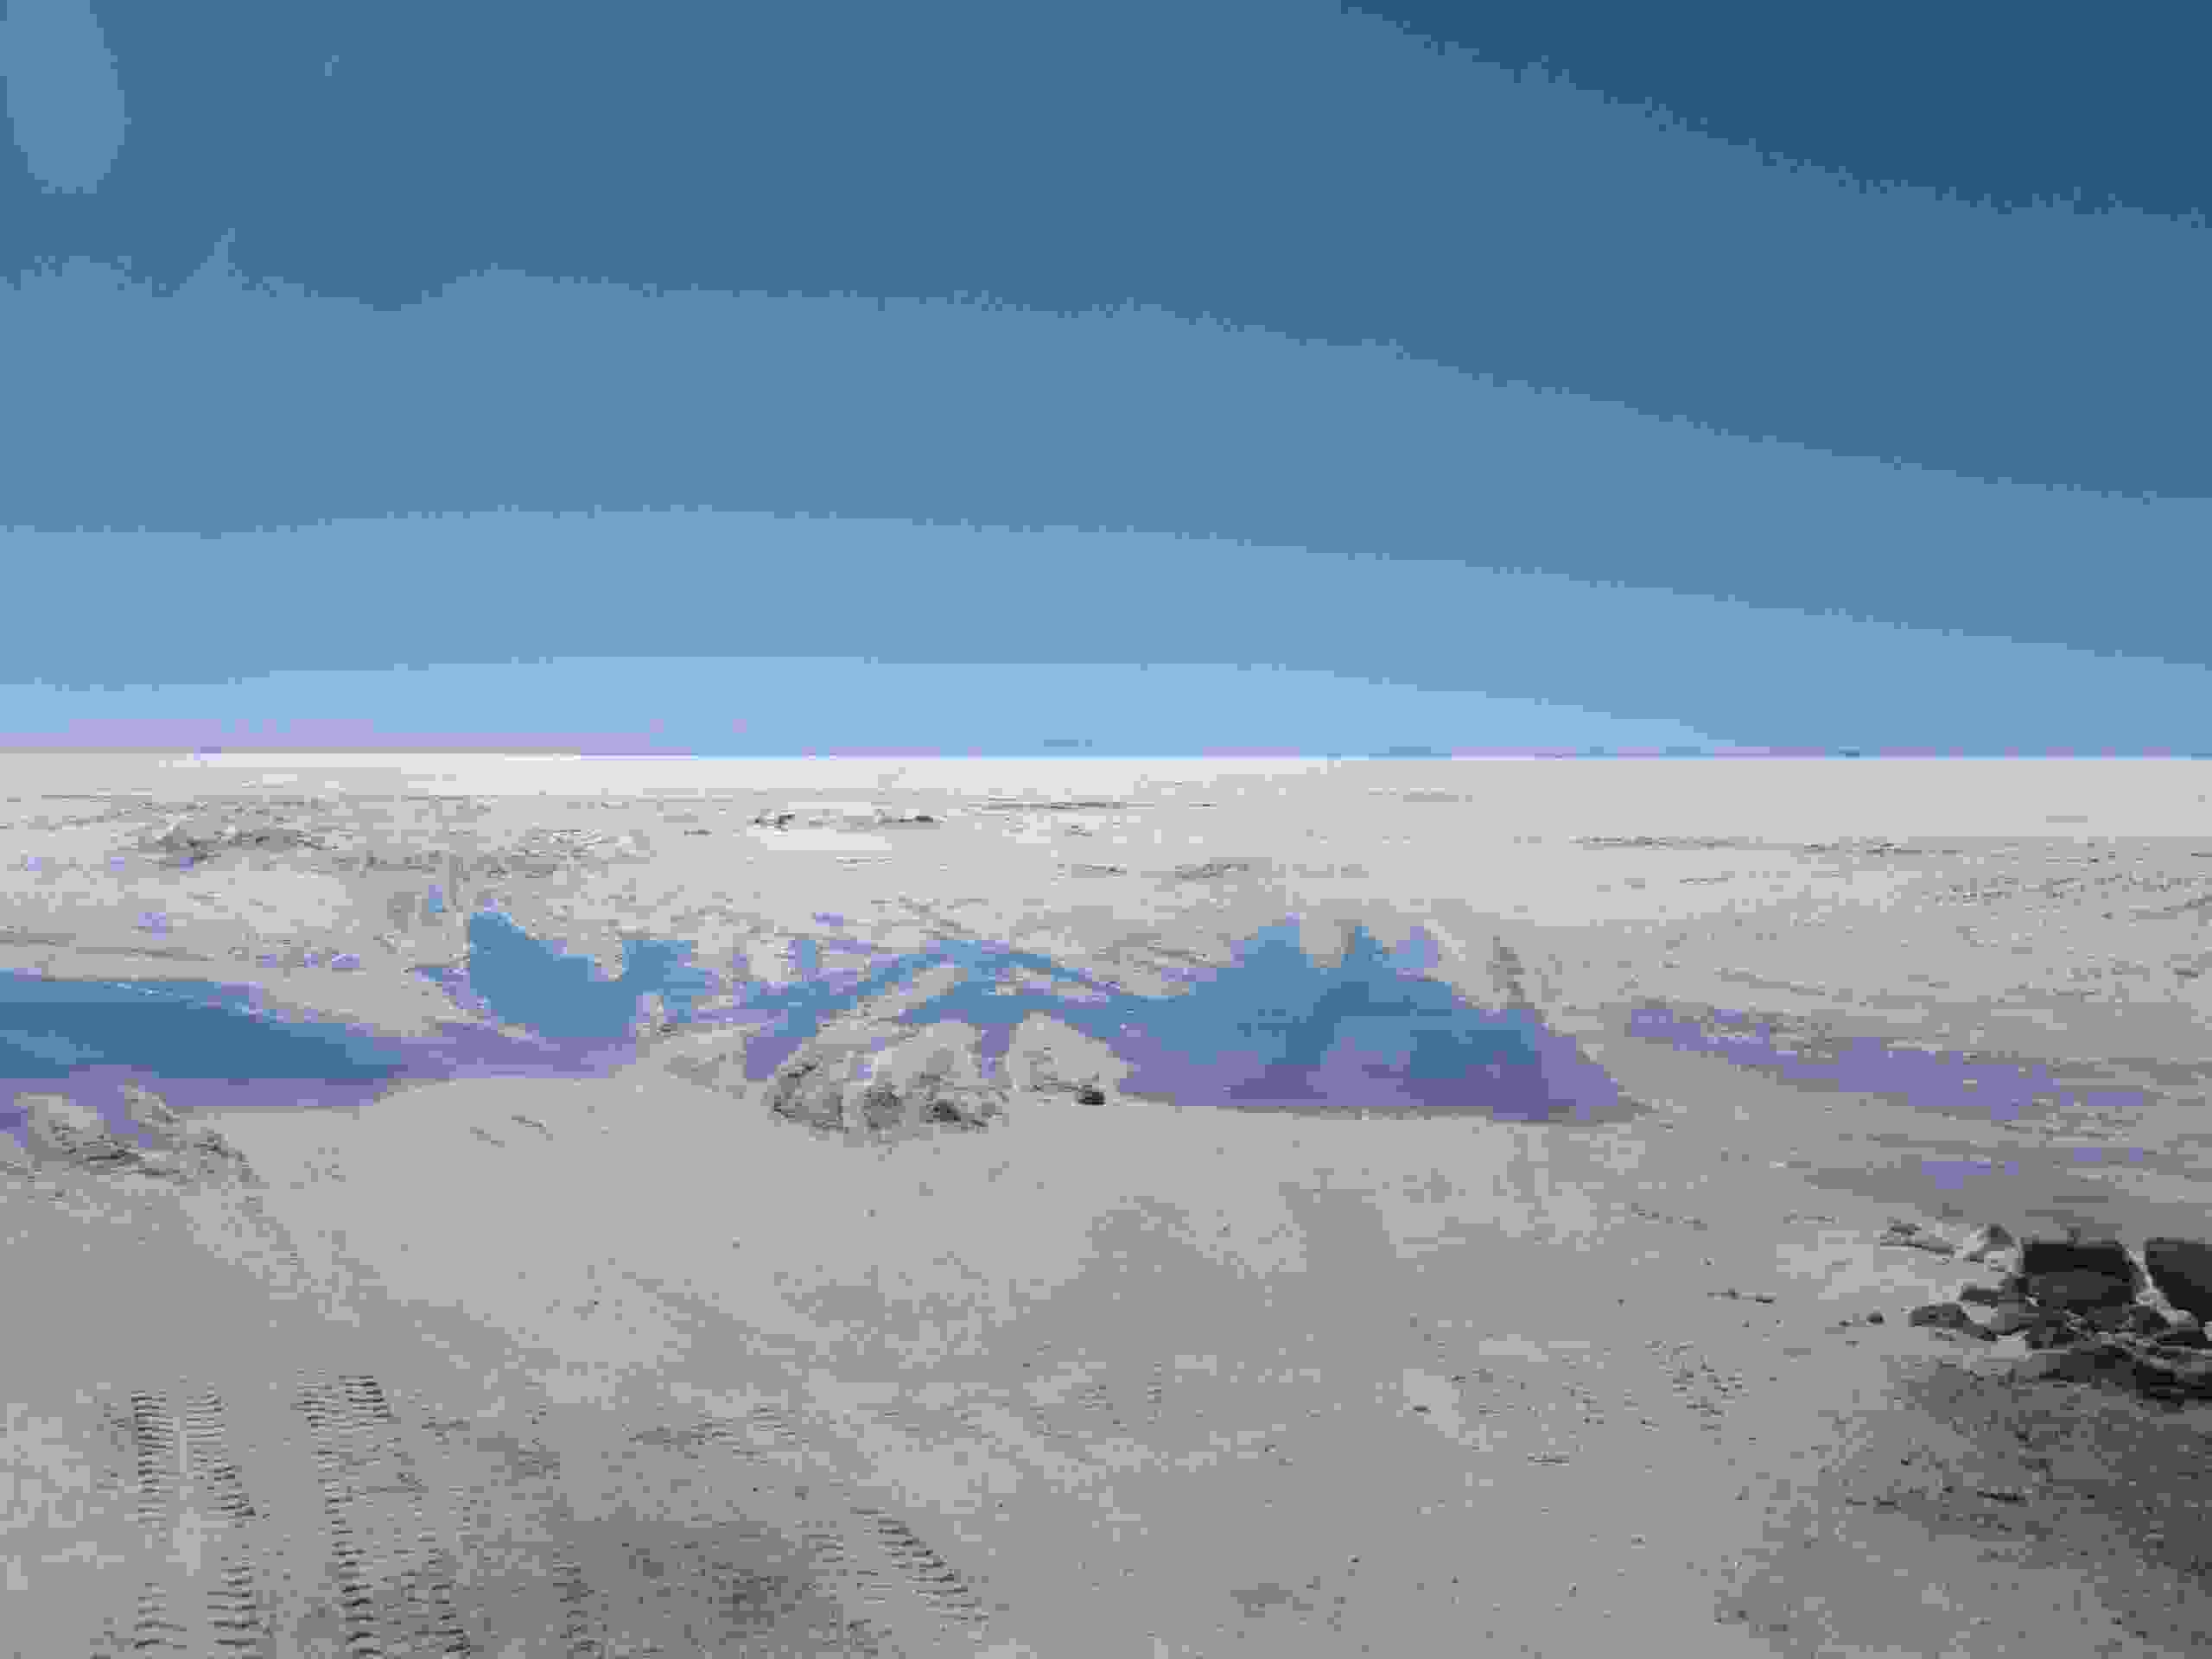
\includegraphics[width=\mywidth]{../wp-content/uploads/2015/04/wpid-wp-1427985949360.jpg} \end{center}



 Puis c'est la traversée, un peu la récompense des efforts passés : environ 70km tout plat et lisse, on peut presque pédaler les yeux fermés !

 

\begin{center} 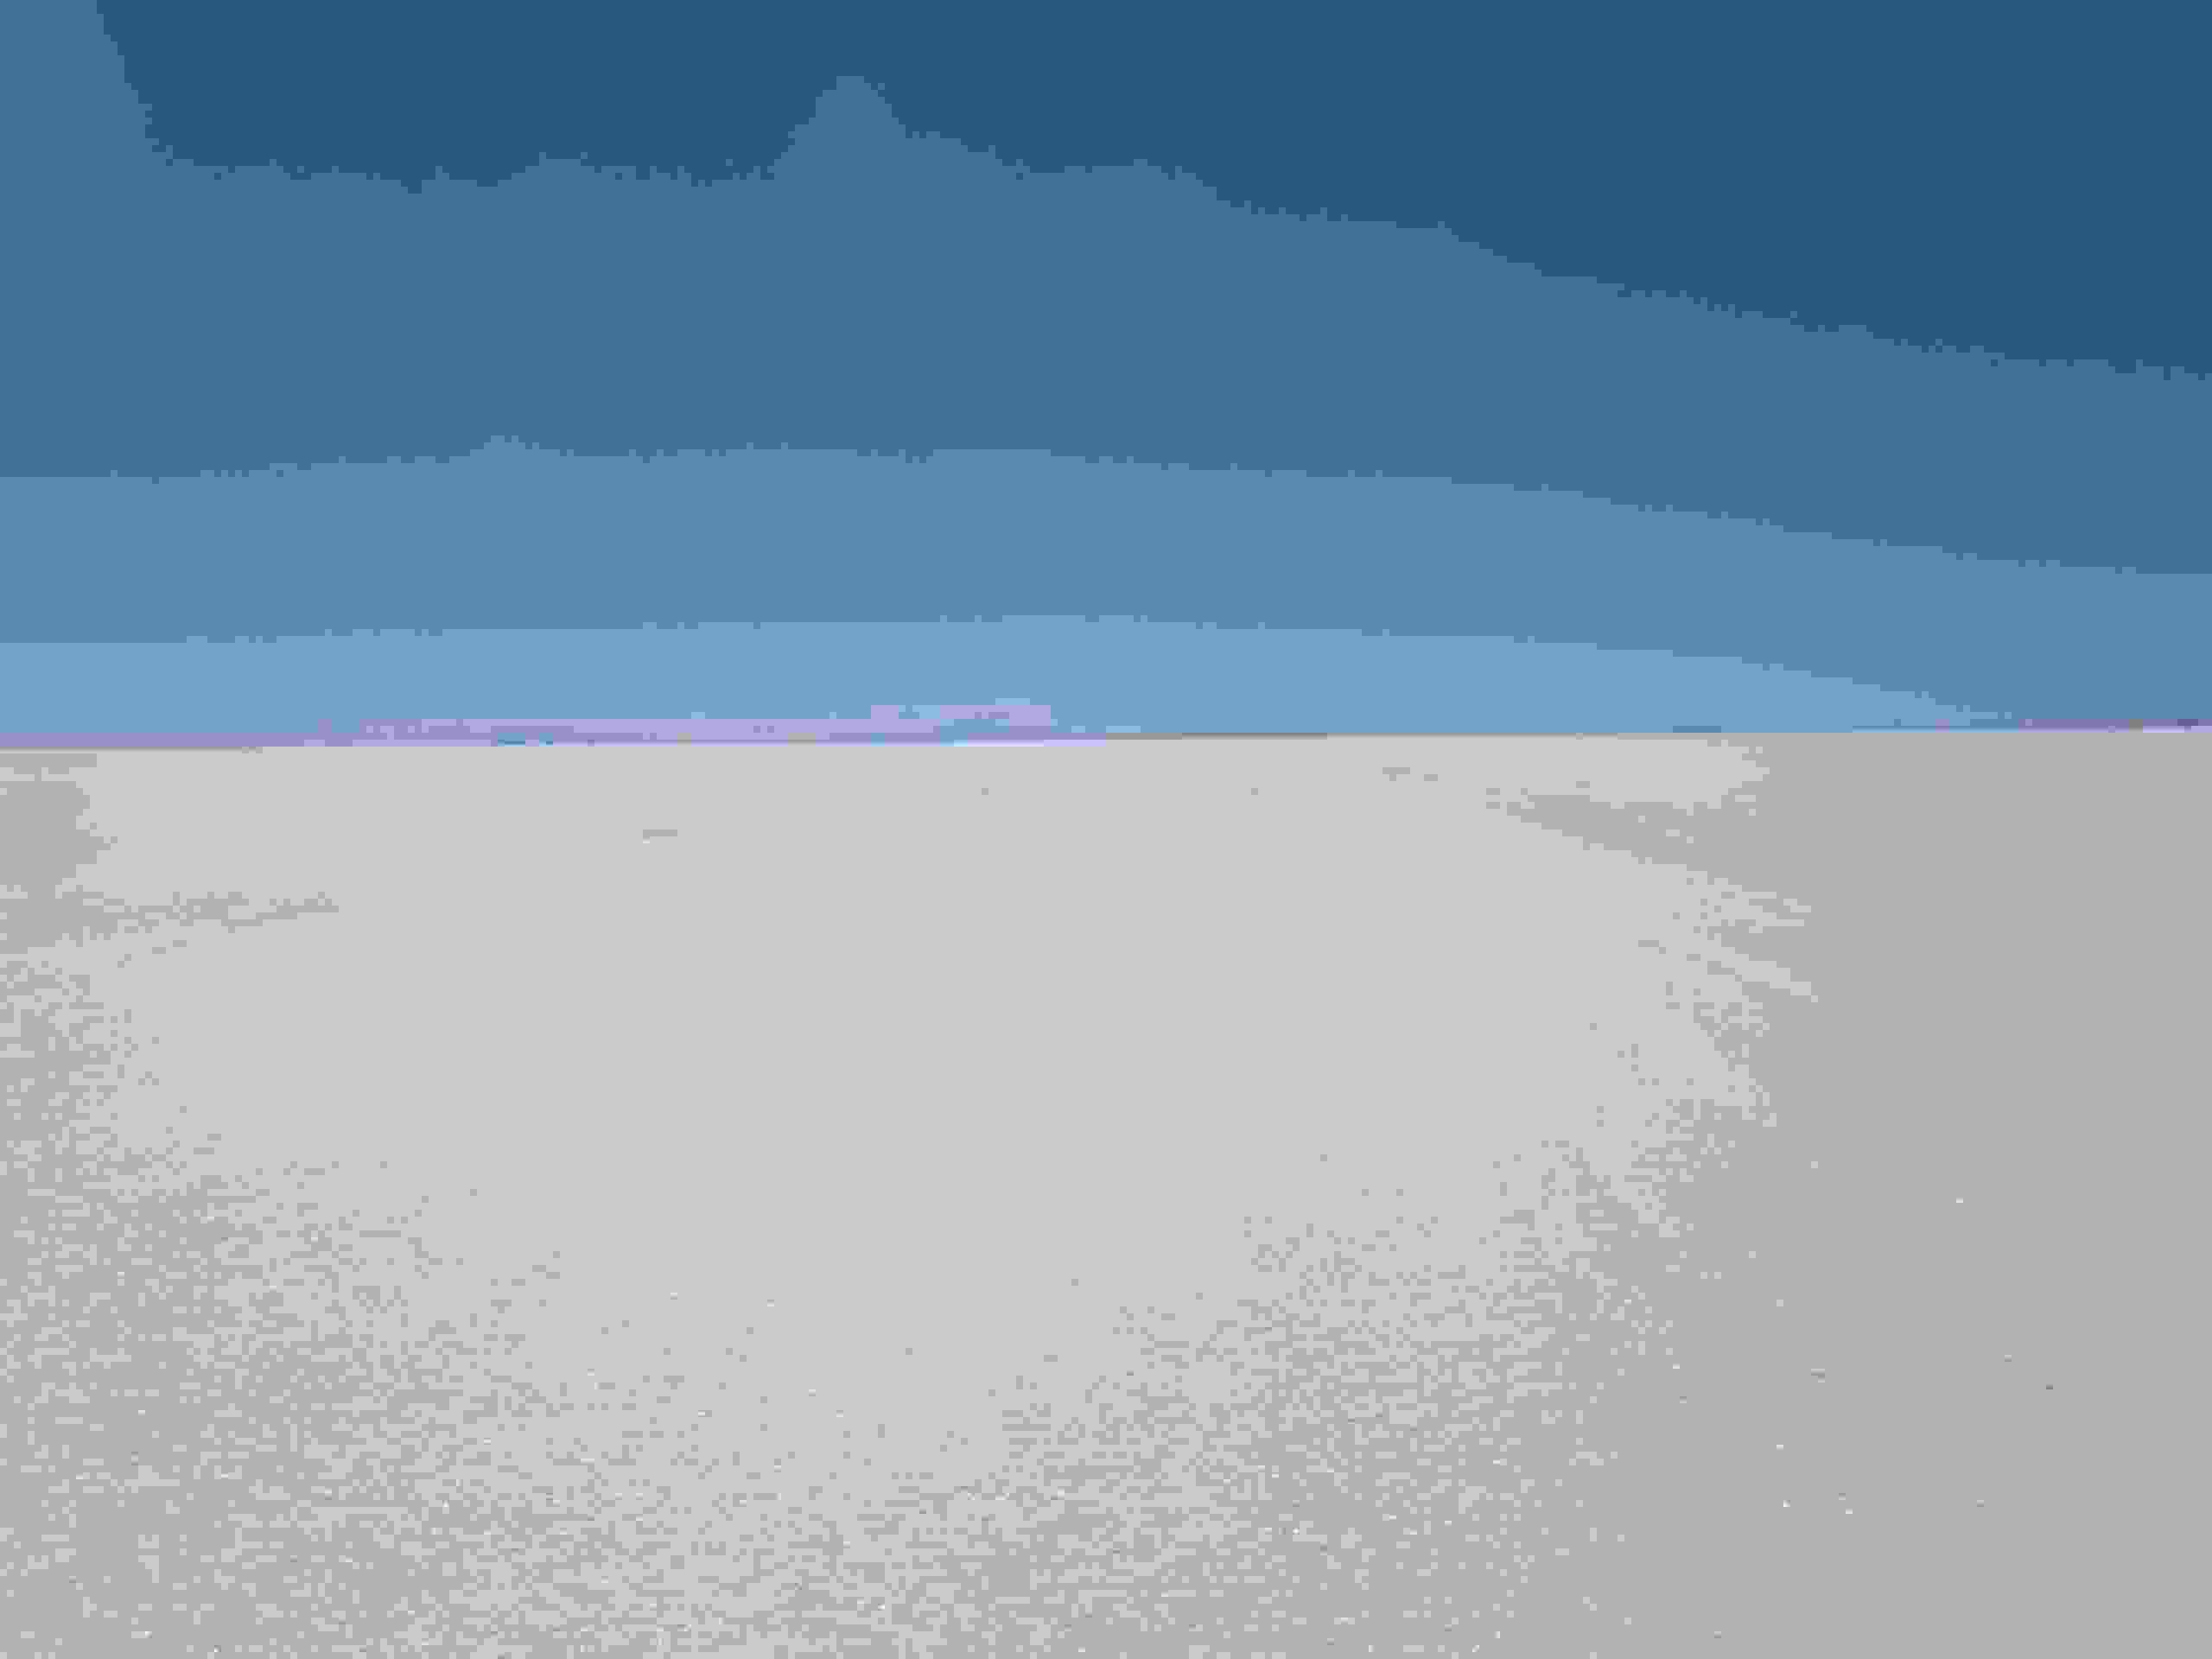
\includegraphics[width=\mywidth]{../wp-content/uploads/2015/04/wpid-wp-1427985961439.jpg} \end{center}



 

\begin{center} 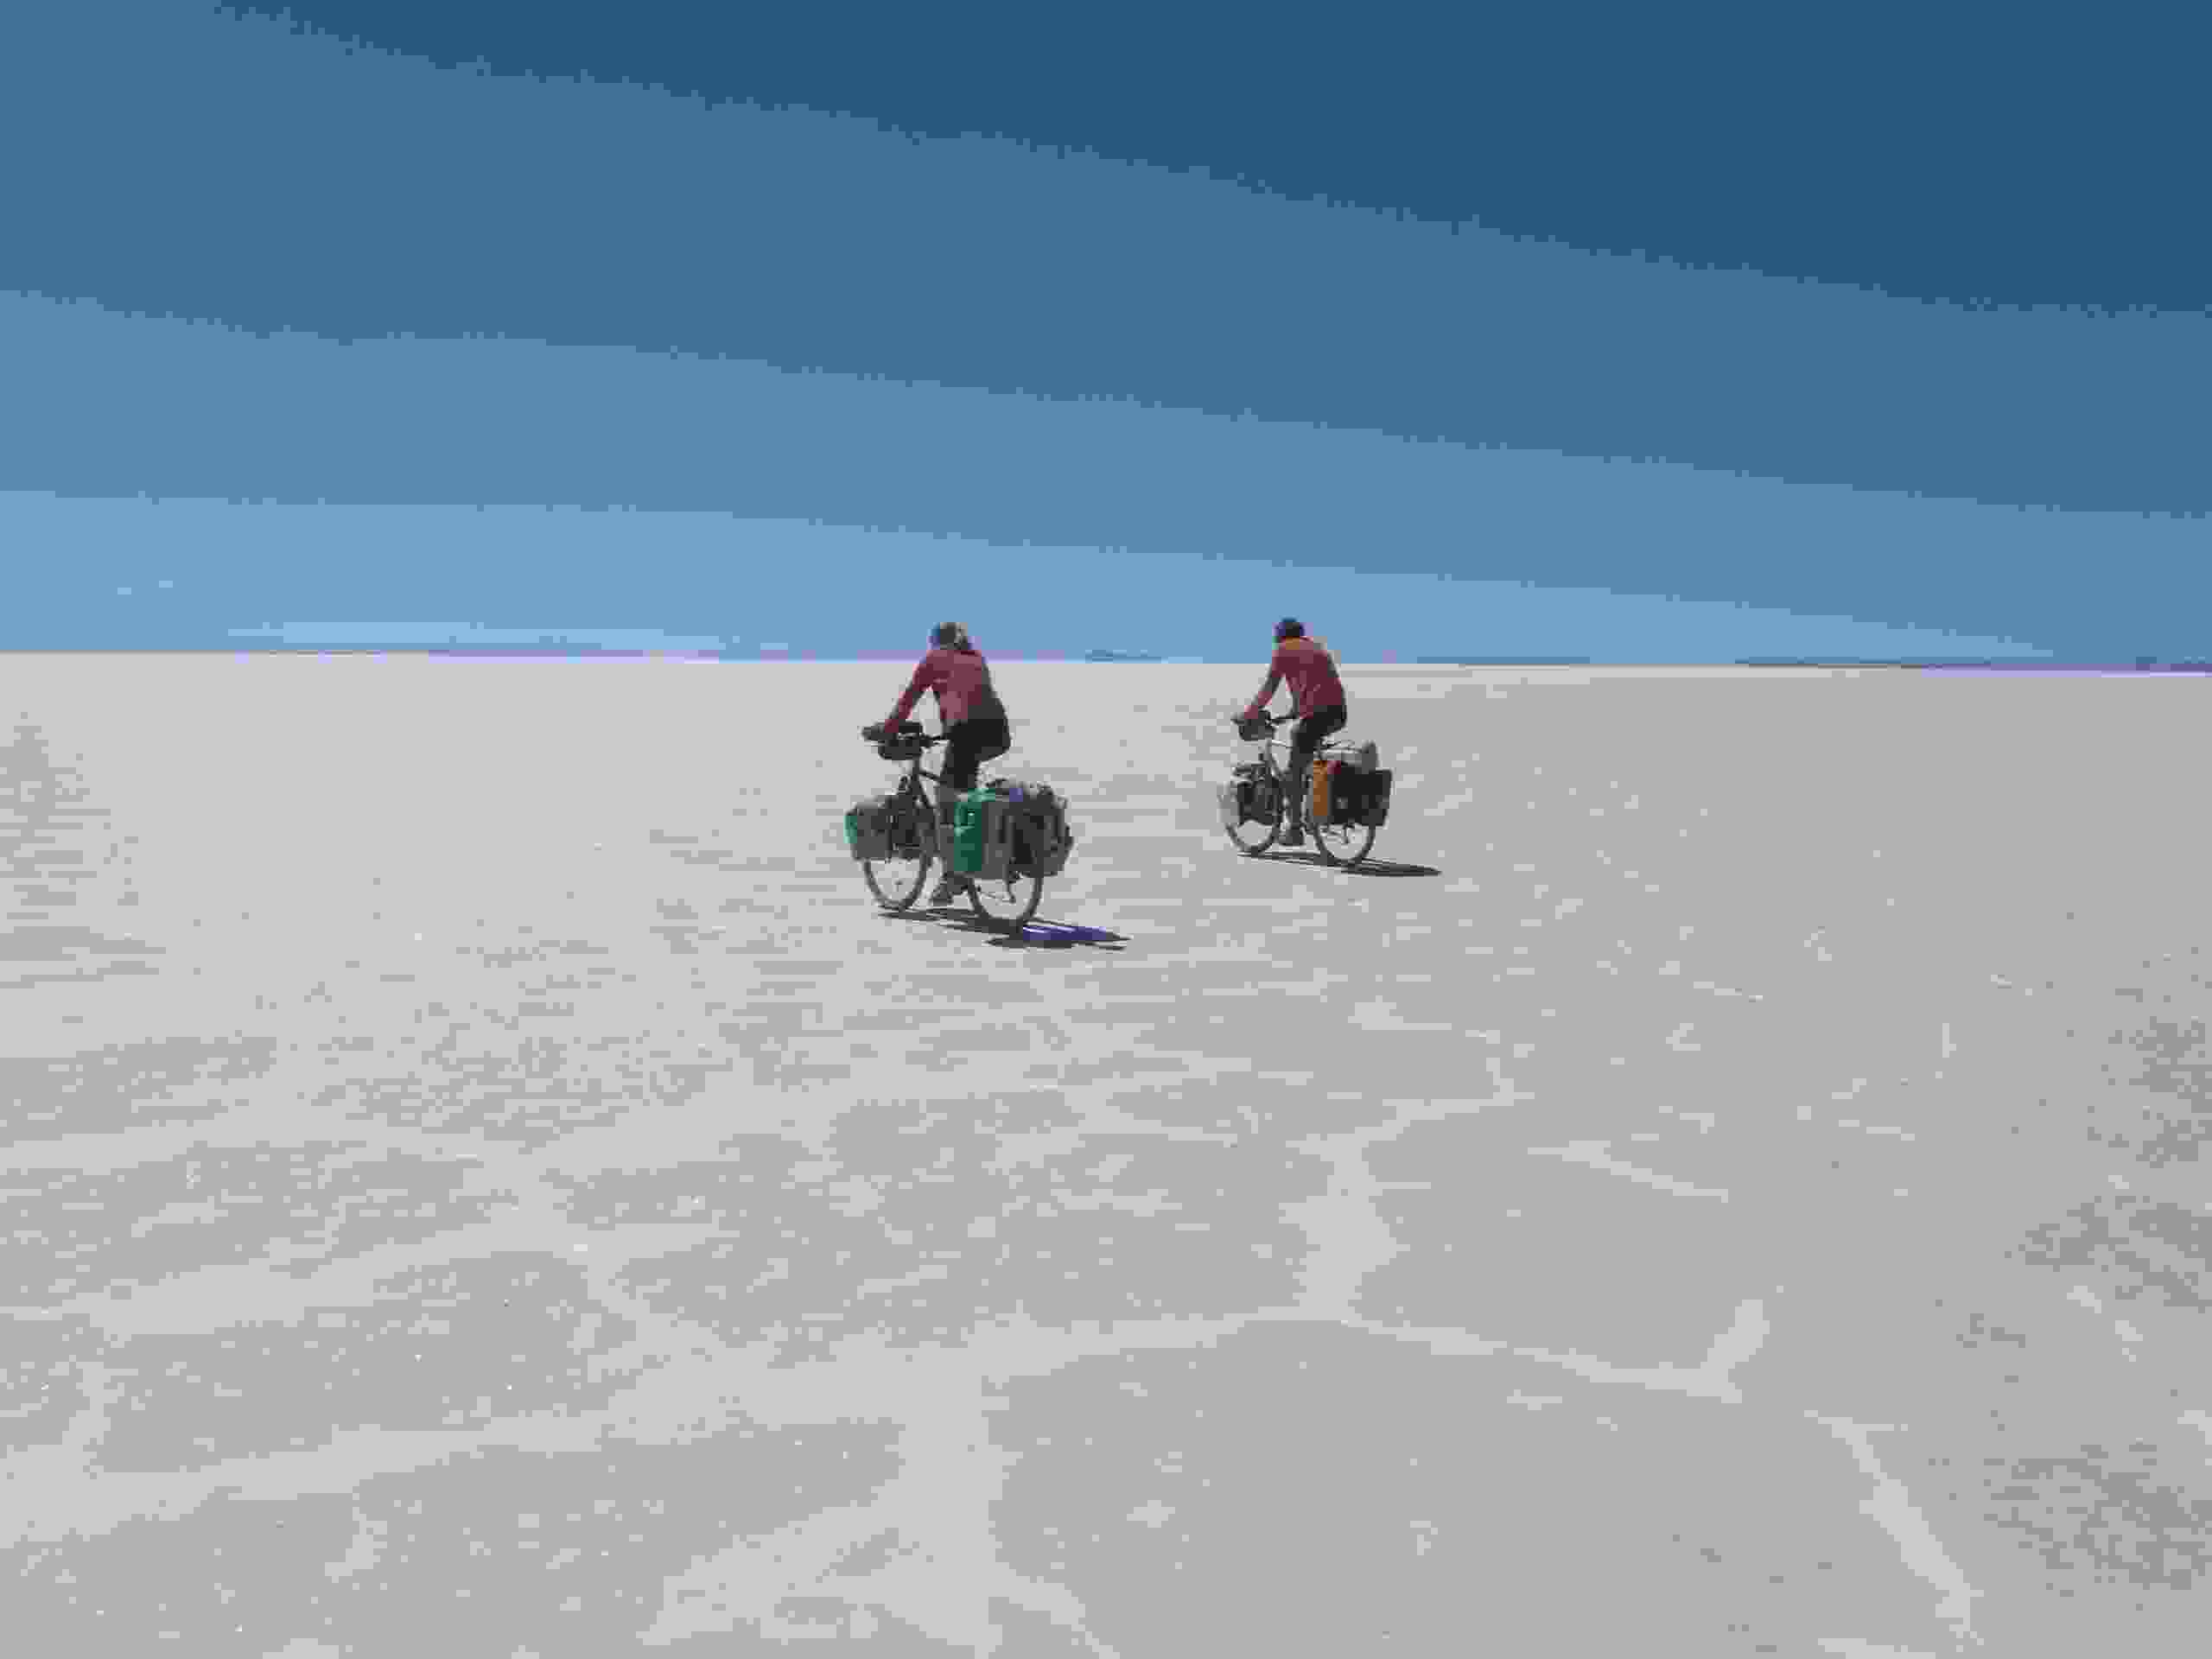
\includegraphics[width=\mywidth]{../wp-content/uploads/2015/04/wpid-wp-1427986094317.jpg} \end{center}



 

\begin{center} 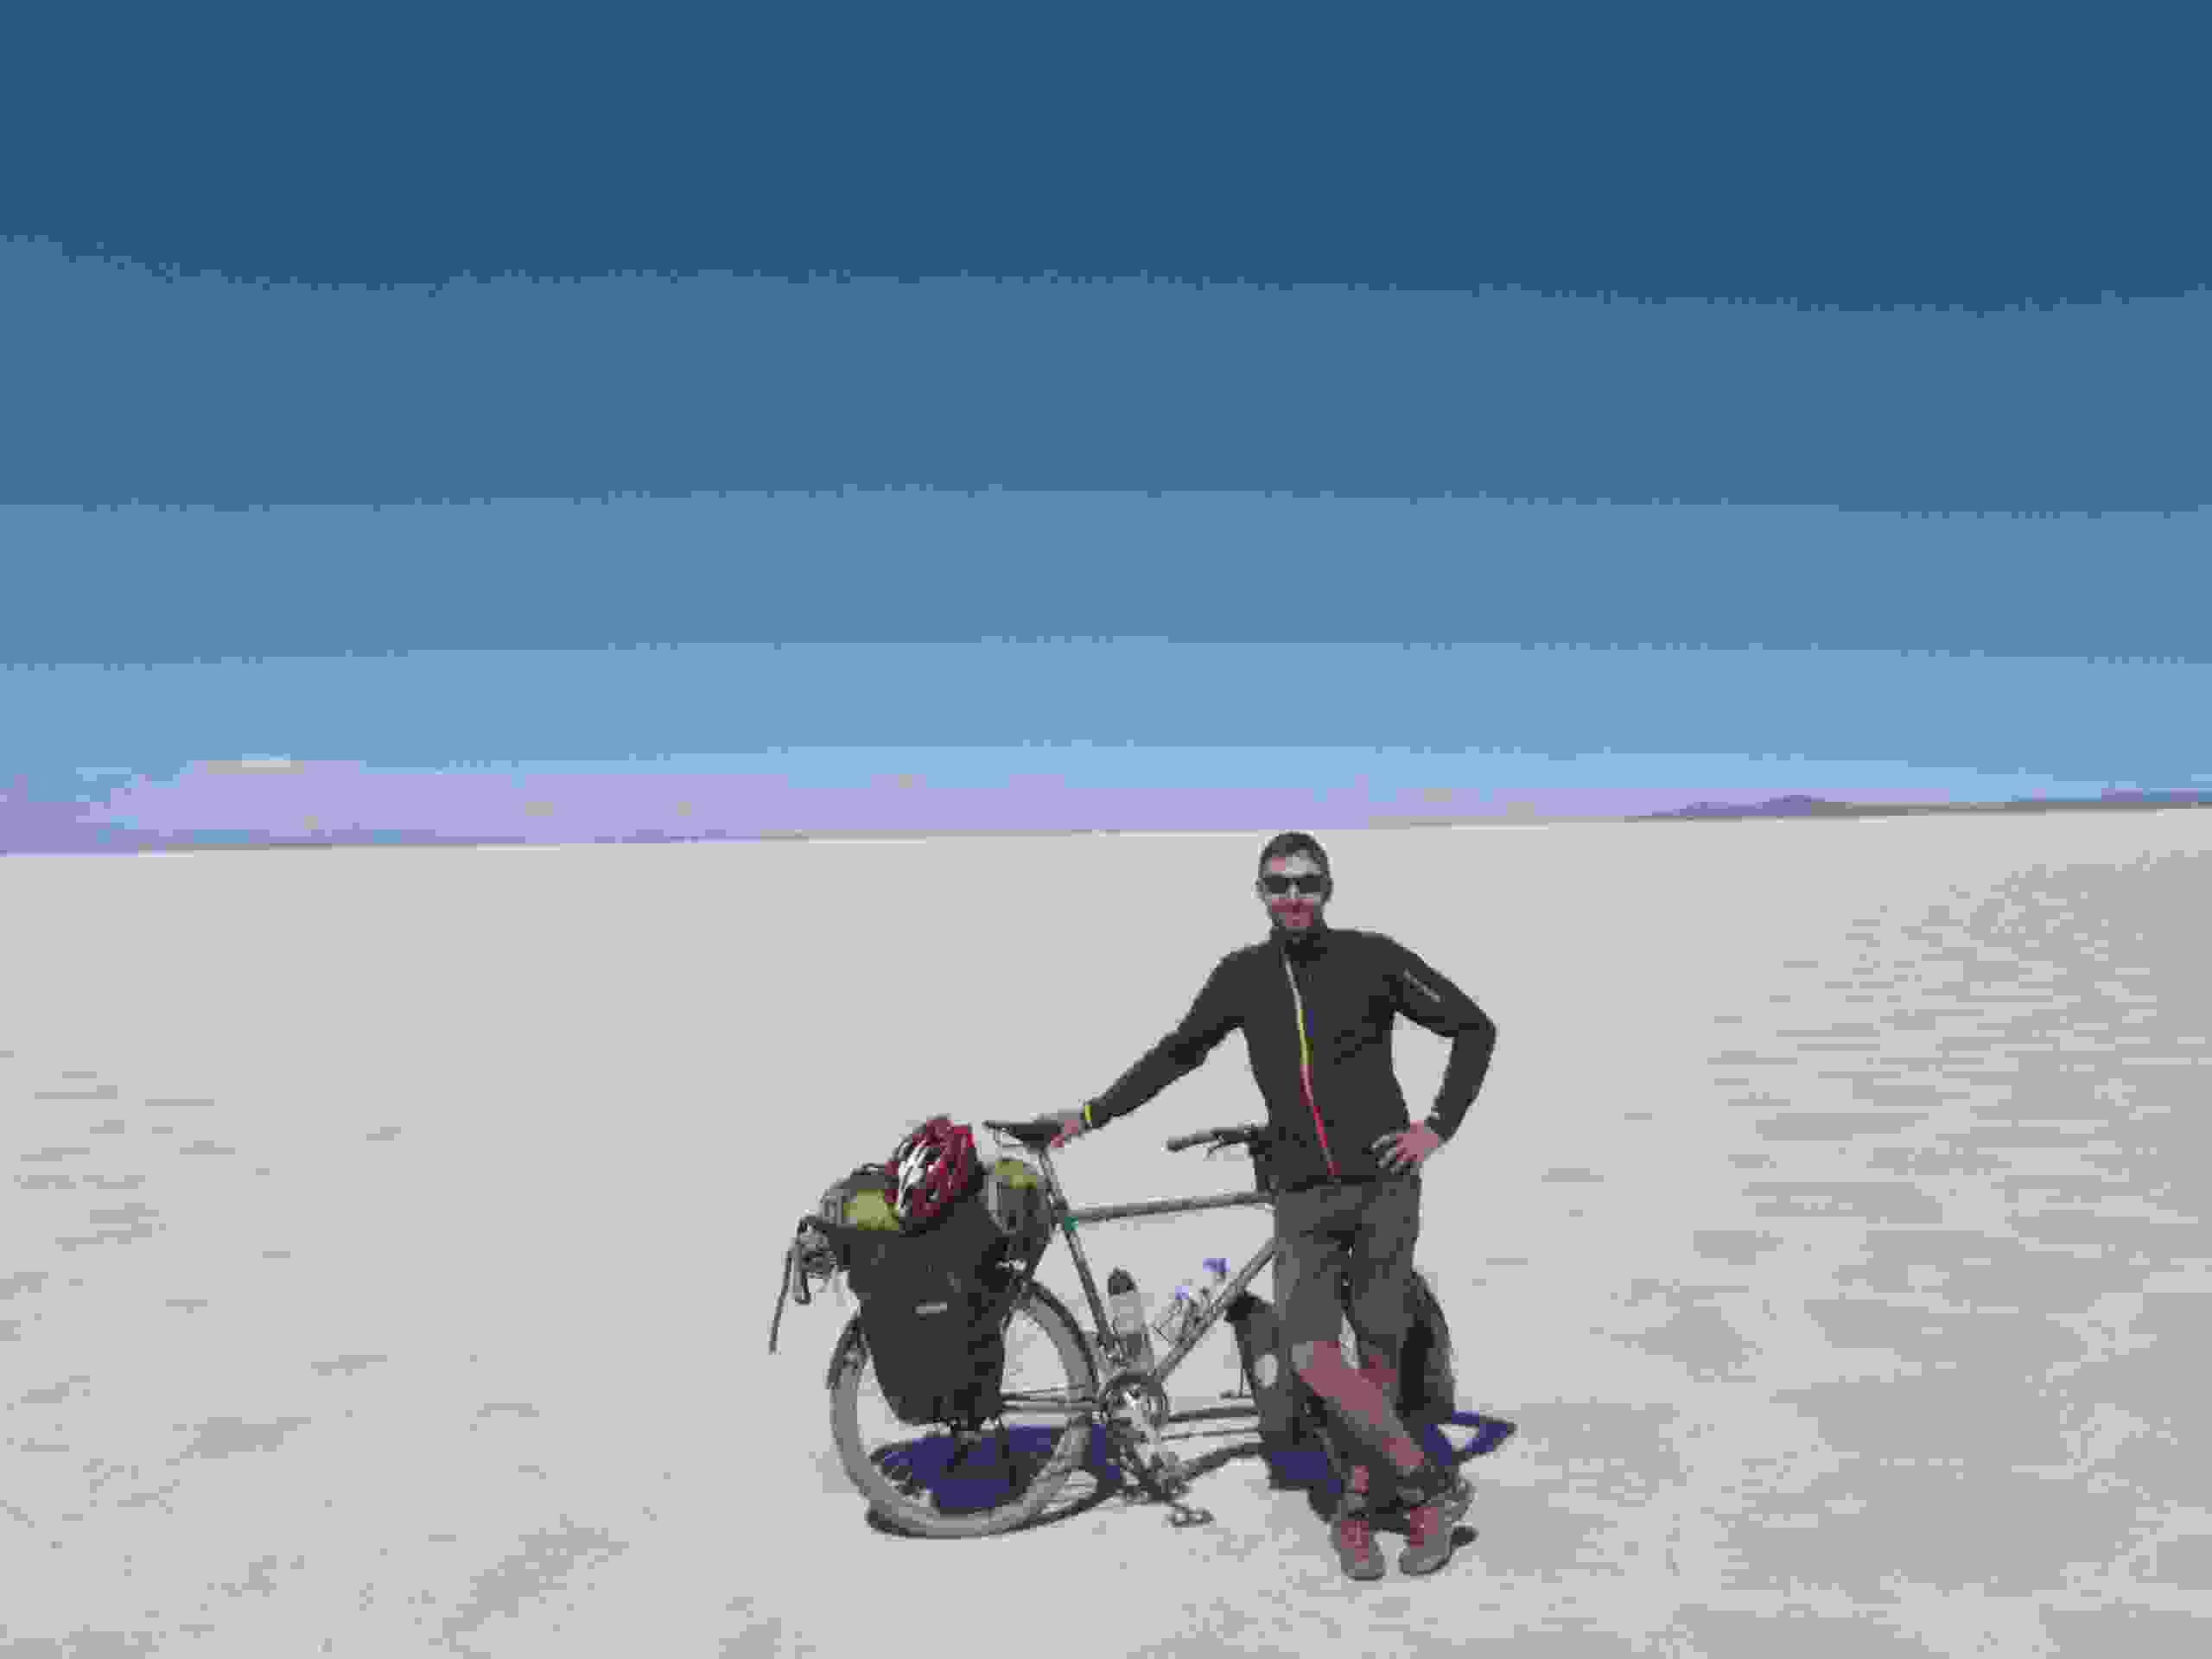
\includegraphics[width=\mywidth]{../wp-content/uploads/2015/04/wpid-wp-1427986011227.jpg} \end{center}



 

\begin{center} 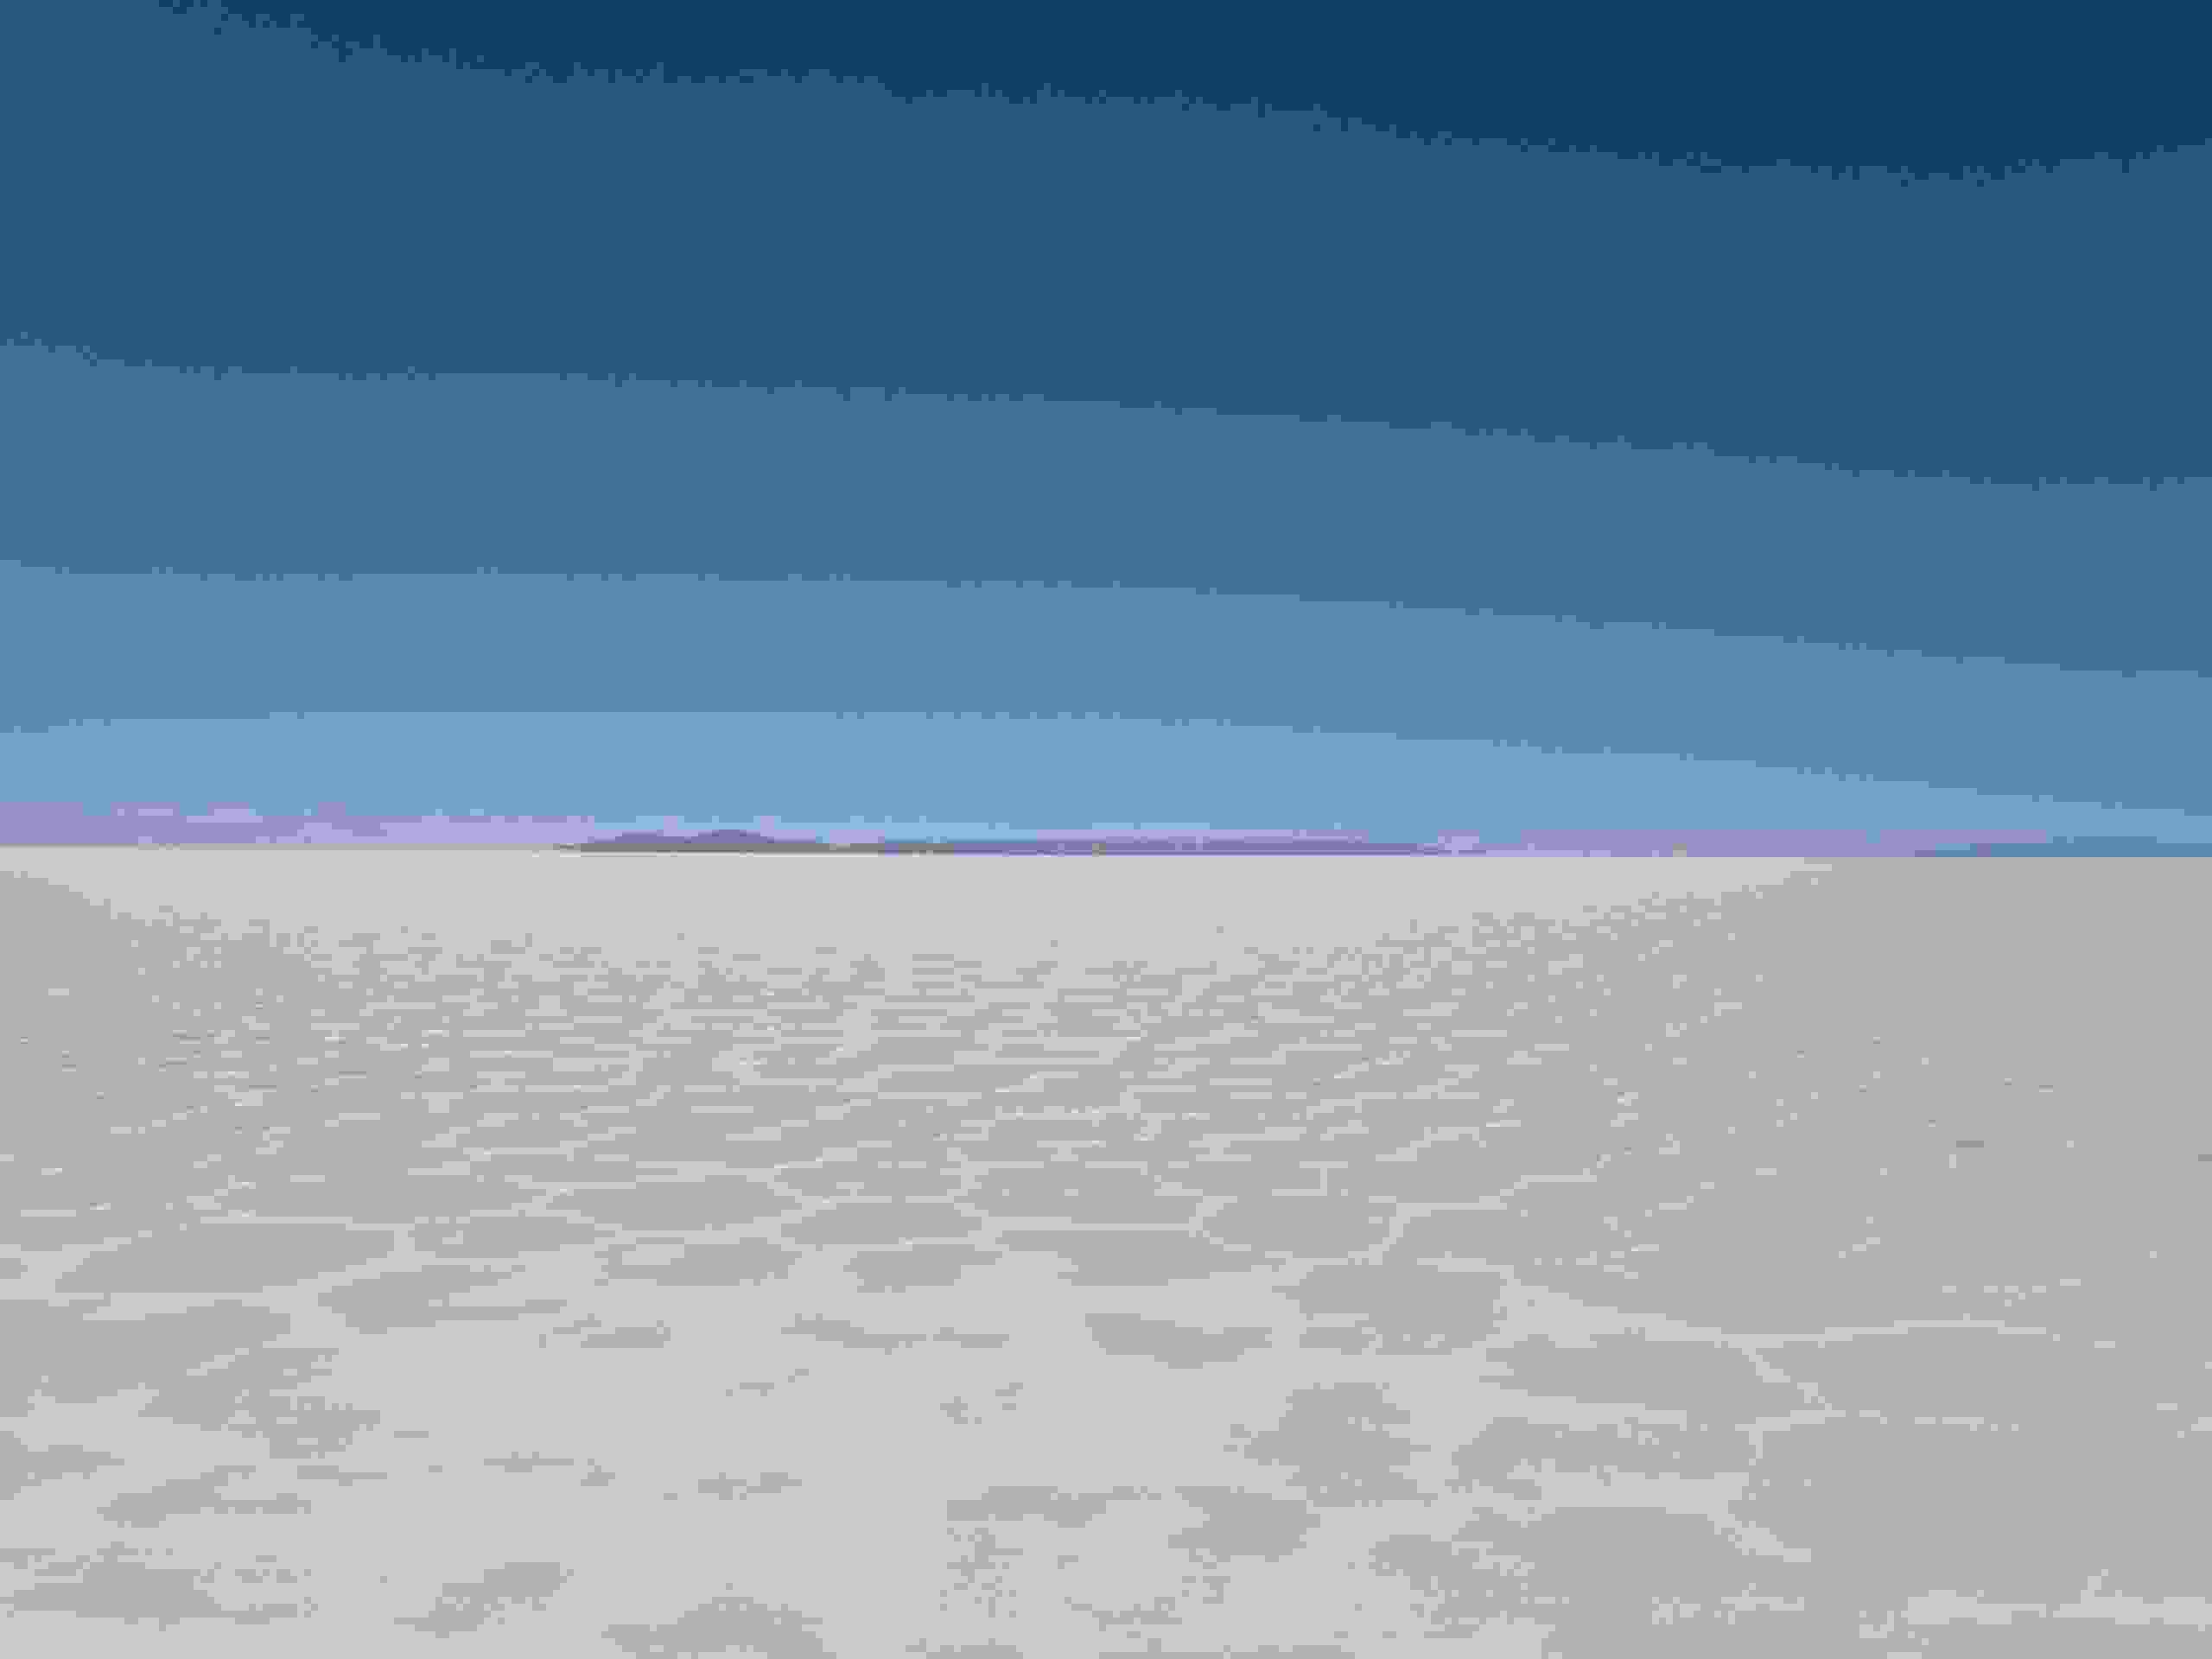
\includegraphics[width=\mywidth]{../wp-content/uploads/2015/04/wpid-wp-1427986063782.jpg} \end{center}



 

\begin{center} 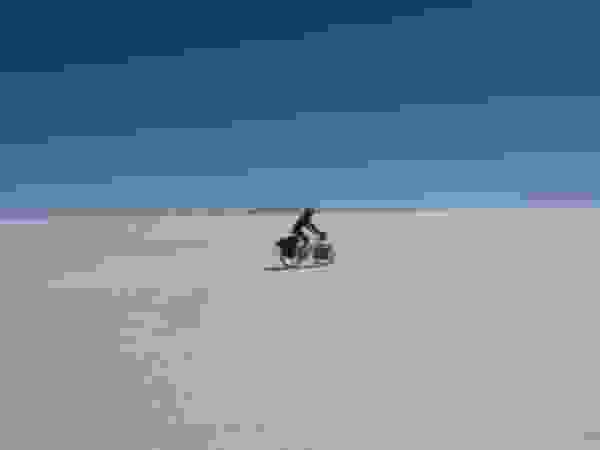
\includegraphics[width=\mywidth]{../wp-content/uploads/2015/04/wpid-p1080201.jpg} \end{center}



 

\begin{center} 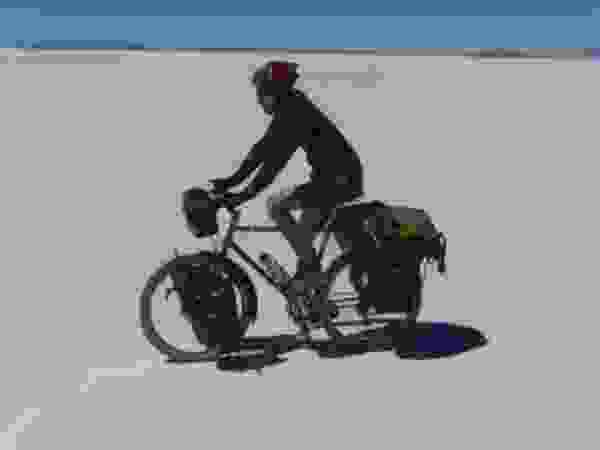
\includegraphics[width=\mywidth]{../wp-content/uploads/2015/04/wpid-p1080206.jpg} \end{center}



 A la sortie du Salar, on rejoint Uyuni pour quelques jours de repos. 

 

\begin{center} 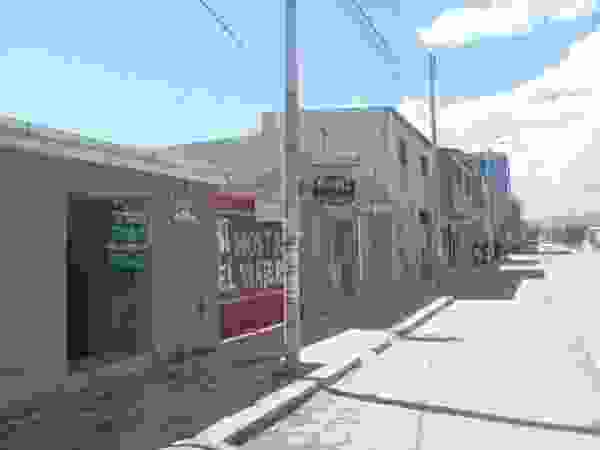
\includegraphics[width=\mywidth]{../wp-content/uploads/2015/04/wpid-wp-1428093286412.jpg} \end{center}



 Le Dakar qui passe dans la région est omniprésent dans la ville. 

 

\begin{center} 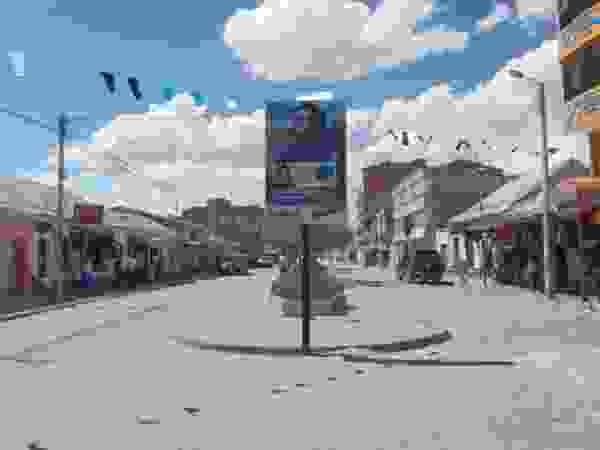
\includegraphics[width=\mywidth]{../wp-content/uploads/2015/04/wpid-wp-1428093361665.jpg} \end{center}



 Le cimetière des trains à quelques kilomètres d'Uyuni. 

 

\begin{center} 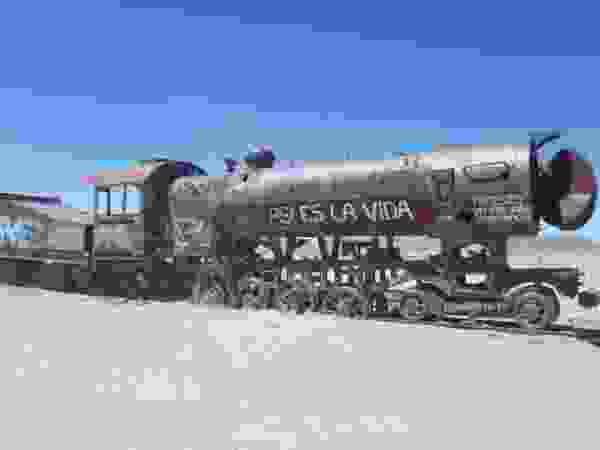
\includegraphics[width=\mywidth]{../wp-content/uploads/2015/04/wpid-wp-1428169906682.jpg} \end{center}



 

\begin{center} 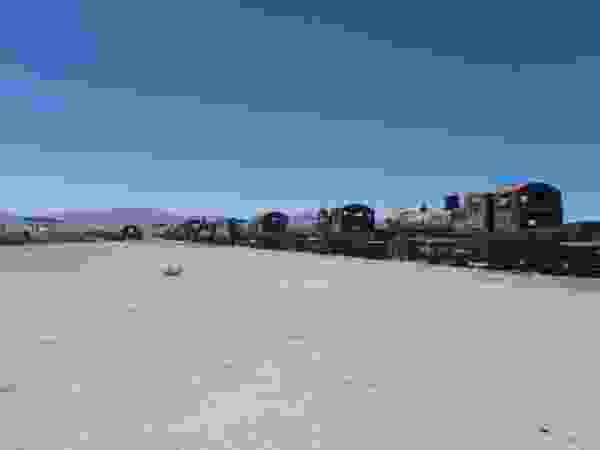
\includegraphics[width=\mywidth]{../wp-content/uploads/2015/04/wpid-wp-1428169937206.jpg} \end{center}



 

\begin{center} 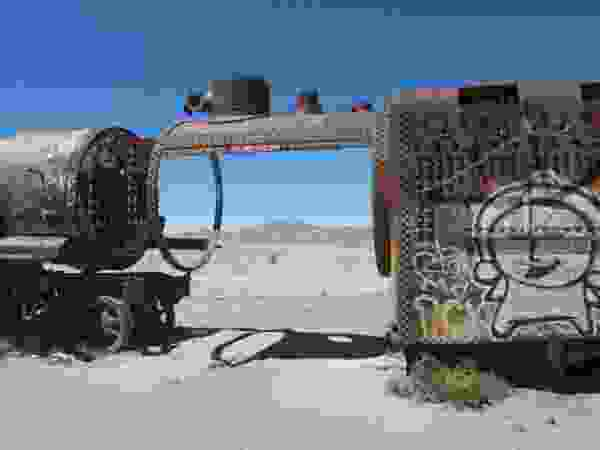
\includegraphics[width=\mywidth]{../wp-content/uploads/2015/04/wpid-wp-1428169957189.jpg} \end{center}



 

\begin{center} 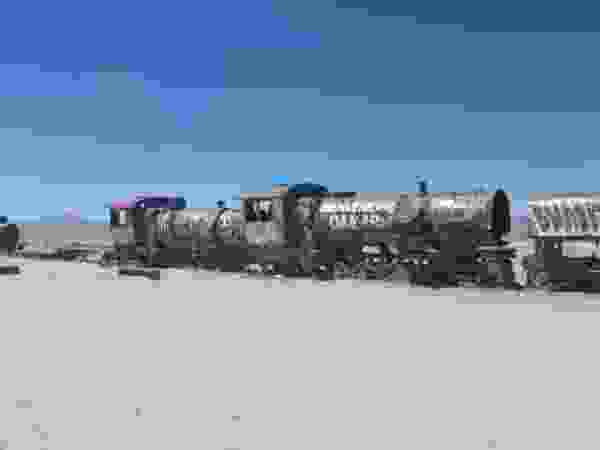
\includegraphics[width=\mywidth]{../wp-content/uploads/2015/04/wpid-wp-1428169984447.jpg} \end{center}




 
 
